\section{Probability Theory}
\begin{frame}{}
\centering	
\Huge{An \textbf{informal} introduction}
    
\end{frame}
\begin{frame}{Probability Spaces}
  \begin{itemize}
    \item A probability space $(\Omega, \mathcal{F}, \mathrm{P})$ consists of:
    \begin{itemize}
      \item $\Omega$: The sample space (set of all possible outcomes).
      \item $\mathcal{F}$: A $\sigma$-algebra, a collection of subsets of $\Omega$ representing events.
      \item $\mathrm{P}$: A probability measure that assigns a number between 0 and 1 to each event in $\mathcal{F}$.
    \end{itemize}
  \end{itemize}
\end{frame}

\begin{frame}[allowframebreaks]{Understanding $\sigma$-Algebra in Simple Terms}
  \begin{itemize}
    \item A $\sigma$-algebra can be understood as defining the \textbf{granularity} of information available.
    \item It must satisfy:
    \begin{itemize}
      \item The whole sample space $\Omega$ is included.
      \item If an event is in $\mathcal{F}$, its complement must also be in $\mathcal{F}$.
      \item If a countable sequence of events is in $\mathcal{F}$, their union must also be in $\mathcal{F}$.
    \end{itemize}

%\input{content/sigmaalg}
    \item Example: Rolling a dice.
    \begin{itemize}
      \item $\Omega = \{1,2,3,4,5,6\}$.
      \item A possible $\sigma$-algebra: $\{\emptyset, \Omega, \{1,3,5\}, \{2,4,6\}\}$ (representing even and odd outcomes).
    \end{itemize}
  \end{itemize}

\framebreak
\begin{figure}
\centering
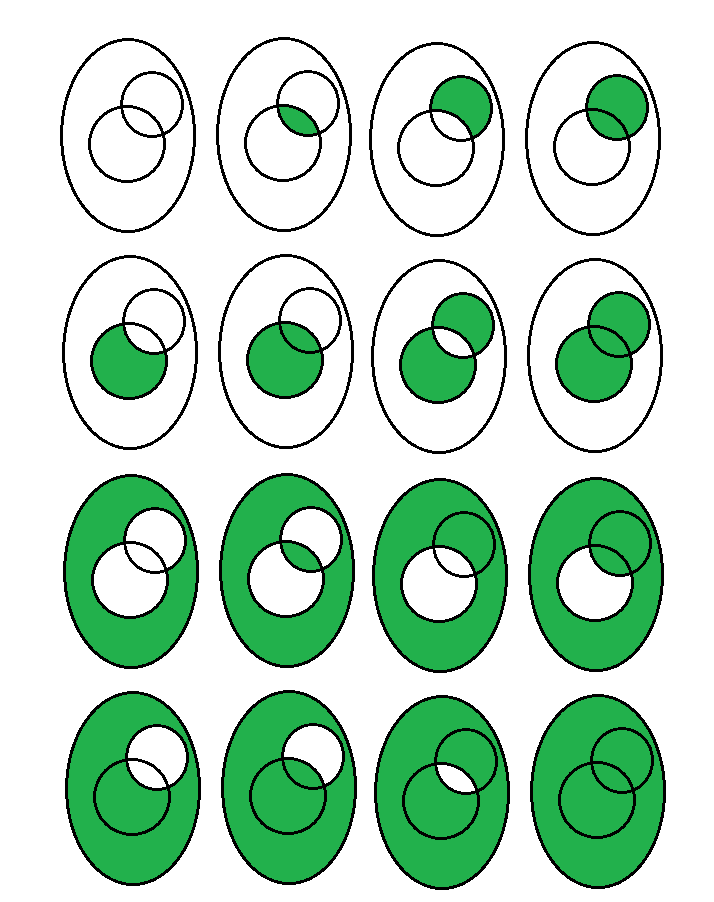
\includegraphics[scale=.3]{figures/sigmaalg.png}
    \caption{Example of $\sigma-$algebra}
    \label{fig:enter-label}
\end{figure}

\end{frame}

\begin{frame}[allowframebreaks]{Random Variables as Mappings}
  \begin{itemize}
    \item A random variable $X$ is a function that maps outcomes from the sample space $\Omega$ to real numbers:
    \begin{equation}
      X: \Omega \to \mathbb{R}
    \end{equation}
    \item Example 1: Rolling a dice.
    \begin{itemize}
      \item Let $X$ be the outcome of a single roll.
      \item If $\omega$ is an element of $\Omega = \{1,2,3,4,5,6\}$, then $X(\omega) = \omega$.
    \end{itemize}
    \item Example 2: Defining an odd/even variable.
    \begin{itemize}
      \item Define $Y(\omega) = 1$ if $\omega$ is odd, and $Y(\omega) = 0$ if $\omega$ is even.
      \item $Y$ maps outcomes to a simpler representation (odd/even classification).
    \end{itemize}
    \framebreak
    \item A random variable must be measurable with respect to a given $\sigma$-algebra to be well-defined.
  %  \item This means that the preimage of any measurable subset of $\mathbb{R}$ must be in the $\sigma$-algebra.
    \item Example:
    \begin{itemize}
      \item With the previously defined $\sigma$-algebra $\{\emptyset, \Omega, \{1,3,5\}, \{2,4,6\}\}$, $Y$ (odd/even) is measurable.
      \item However, $X$ (exact roll outcome) is not measurable under this $\sigma$-algebra since it distinguishes between individual numbers. A \textbf{finer} sigma-algebra is needed: $\sigma(\{\{1\},\{2\},\{3\},\{4\},\{5\},\{6\}\})$.
    \end{itemize}
    \item An intuitive interpretation of measurability comes from \textbf{Doob's lemma}: A random variable is measurable with respect to a $\sigma$-algebra if and only if there exists a function that depends only on elements of the algebra.
   % \item This means that if we only know events from a given $\sigma$-algebra, we can still determine the value of the measurable random variable using some function of those events.
  \end{itemize}
\end{frame}

\section{Stochastic Processes}

\begin{frame}{Introduction to Stochastic Processes}
  \begin{itemize}
    \item A stochastic process is a collection of random variables indexed by time:
    \begin{equation}
      Y_t: \Omega \to \mathbb{R}, \quad t \geq 0
    \end{equation}
    \item It describes how a system evolves randomly over time.
    \item Examples:
    \begin{itemize}
      \item Stock prices.
      \item Population dynamics.
      \item Temperature variations.
    \end{itemize}
  \end{itemize}
\end{frame}



\begin{frame}{Filtration and Adapted Processes}
  \begin{itemize}
    \item A filtration is a sequence of $\sigma$-algebras representing growing information over time:
    \begin{equation}
      \mathcal{F}_0 \subseteq \mathcal{F}_1 \subseteq \mathcal{F}_2 \subseteq \dots
    \end{equation}
    \item Intuitively, it models the \textbf{accumulation of knowledge} as time progresses.
    \item A process is adapted if at each time instant is measurable wrt the filtration.
  \end{itemize}


  
\end{frame}

\begin{frame}{Probability measure}

({\color{red}\textbf{Informal, not complete}}) In the framework of measure theory, a probability measure $\mu$ is a mapping from \textbf{subsets} $\{S_i\}_i$ of a given sample space $\Omega$ such that:
\begin{itemize}
    \item It is positive $\mu(S_i)\geq 0$
    \item For disjoint sets $S_i,S_j$ ($S_i\cap S_j=\emptyset$)it holds $\mu(S_i\cup S_j)=\mu(S_i)+\mu( S_j)$. (Actual definition: extension to countable unions of pairwise disjoint sets)
    \item Its "\textit{integral}" is equal to one ($\mu(\Omega)=1$).
\end{itemize}

Familiar examples:
\begin{itemize}
    \item $\Omega=\mathrm{R}$, Gaussian probability $\mu(dx)=p(x)dx=\frac{1}{\sqrt{2\pi}}\exp(-\frac{x^2}{2})dx$
    \item $\Omega=\{0,1\}$, Bernoully RV $\mu(\{0\})=\mu(\{1\})=\frac{1}{2}$
\end{itemize}
    
\end{frame}
\begin{frame}[allowframebreaks]{Definition of SDEs}
  
  \begin{itemize}
    \item A stochastic differential equation (SDE) is a particular class of stochastic processes.
\item A general diffusion process on a probability space $(\Omega, \mathcal{F}, \mathrm{P})$ is given by:
  \begin{equation}
      Y_t(\omega) = Y_0(\omega) + \int_0^t H(Y_s(\omega),t)\dd s + W_t(\omega)
  \end{equation}
  where:
  \begin{itemize}
    \item $Y_t$ is the stochastic process.
    \item $H(Y_t(\omega),t)$ is the drift term.
    \item $W_t$ is a Brownian motion, representing Gaussian noise.
  \end{itemize}
      \item As discussed before, it only makes sense when considered with respect to a \textbf{filtration} $(\mathcal{F}_t)_{t \geq 0}$, which represents the available information over time.
  \end{itemize}

  
\end{frame}


\begin{frame}[allowframebreaks]{Introduction}
\begin{itemize}
\item Consider a probability space $(\Omega,\mathcal{F},\mathbb{P})$, together with a growing filtration $\mathcal{F}_t$
    \item Consider a generic random variable $A$ ($\mathcal{F}_0$-measurable) with probability measure $\mu^A(\dd x)$
    \item Build a simple SDE in $[0,T]$ with initial conditions $\sim \mu^A$
    \begin{equation}\label{eq:diffsdes}
    \begin{cases}
    \dd X_t=-X_t\dd t+\sqrt{2}\dd W_t,\\
    X_0=A\sim \mu^A
    \end{cases}
\end{equation}
where $W_t$ is an $\mathcal{F}_t$ Brownian motion.
    \item This SDE corresponds to a path measure $\mathbb{P}^{A}$. Precise definition requires defining sigma-algebra generated by the stochastic process $X_{0\leq t\leq T}$.
\item Two SDEs which differ only by initial conditions have KL divergence 

\begin{equation}
 \KL{\mathbb{P}^{{\mu^A}}}{\mathbb{P}^{{\mu^B}}}=\E_{\mathbb{P}^{{\mu^A}}}\left[\log\frac{\dd\mathbb{P}^{{\mu^A}}}{\dd\mathbb{P}^{{\mu^B}}}\right]=\E_{\mathbb{P}^{{\mu^A}}}\left[\log\frac{\dd \mu^{A}}{\dd p^{B}}\right]=\KL{\mu^A}{\mu^B}  
\end{equation}
\item Disintegration of measures explains why (simply Markov): $\frac{\dd \mathbb{P}^{\mu^{A}}}{\dd \mathbb{P}^{\mu^{B}}} (\omega)=\frac{\dd \left(\mathbb{P}^{\mu^A}\#_{\omega_{0}}\right)}{\dd \left(\mathbb{P}^{\mu^B}\#_{\omega_{0}}\right)} (\omega)\frac{\dd \mu^A(\omega_{0})}{\dd \mu^B(\omega_{0})}=\frac{\dd \mu^A(\omega_{0})}{\dd \mu^B(\omega_{0})}$
\end{itemize}  
\framebreak
\textbf{Time-reversal} $\hat{X}_t\defeq X_{T-t}$:
\begin{itemize}
    \item KL between path measures is invariant to time-reversal $\KL{\mathbb{P}^{{\mu^A}}}{\mathbb{P}^{{\mu^B}}}=\KL{\hat{\mathbb{P}}^{{\mu^A}}}{\hat{\mathbb{P}}^{{\mu^B}}}$
    \item Time reversal of SDE is again an SDE (provided technical conditions [ Leonard 2014])
    \begin{equation}
         \dd \hat X_t=\hat X_t+2 \underbrace{\nabla\log \frac{\dd\mu_{T-t}^A}{\dd \lambda}(\hat X_t)}_{\text{score function!}}\dd t+ \sqrt{2}\dd \hat W_t
    \end{equation}
    with $\lambda$ the Lebesgue measure
    \item Score function $\leftrightarrow$ Denoiser: \begin{equation}
        \nabla\log \frac{\dd\mu_t^A}{\dd \lambda}(x)=\nabla\log p^A_t(x)=\frac{ \exp(-t){\color{red}\E_{{\mathbb{P}^{{\mu^A}}}}[X_0\g X_t=x]}-x}{1-\exp(-2t)}
    \end{equation}
\end{itemize}


\framebreak
\textbf{Girsanov theorem}: (informal) express the KL between path measures corresponding to two \glspl{SDE} with different drifts.

\begin{equation}
  \KL{\hat{\mathbb{P}}^{\mu^{A}}}{\hat{\mathbb{P}}^{\mu^{B}}}\simeq  \E_{   {\mathbb{P}}^{\mu^A}}\left[\int\limits_0^T\norm{\nabla\log p^{A}_t(X_t)-\nabla\log p^{B}_t(X_t) }^2\dd t\right]
\end{equation}
\begin{itemize}
    \item Combining with $\KL{\mathbb{P}^{{\mu^A}}}{\mathbb{P}^{{\mu^B}}}=\KL{\hat{\mathbb{P}}^{{\mu^A}}}{\hat{\mathbb{P}}^{{\mu^B}}}$ we can obtain a KL-estimator!
\item Initial conditions $\KL{\mu^A_T}{\mu^B_T}$ should be negligible (Bakry-Emery condition of diffusion semigroup or in layman terms, ergodicity [Collet, Florent Malrieu, 2008]. Log-Sobolev ineq. for inhomogeneous
Markov semigroups)
\end{itemize}

\end{frame}


\section{Results}



\begin{frame}[allowframebreaks]{Experimental Results}
%\input{content/table}
%\framebreak
MINDE variants:
\begin{itemize}
    \item Consistently outperform all competitors on standard benchmarks.
    \item Are capable of accurately estimating MI in the challenging High MI benchmarks:
\begin{figure}[ht]
    \centering
    \begin{subfigure}{0.25\textwidth}
        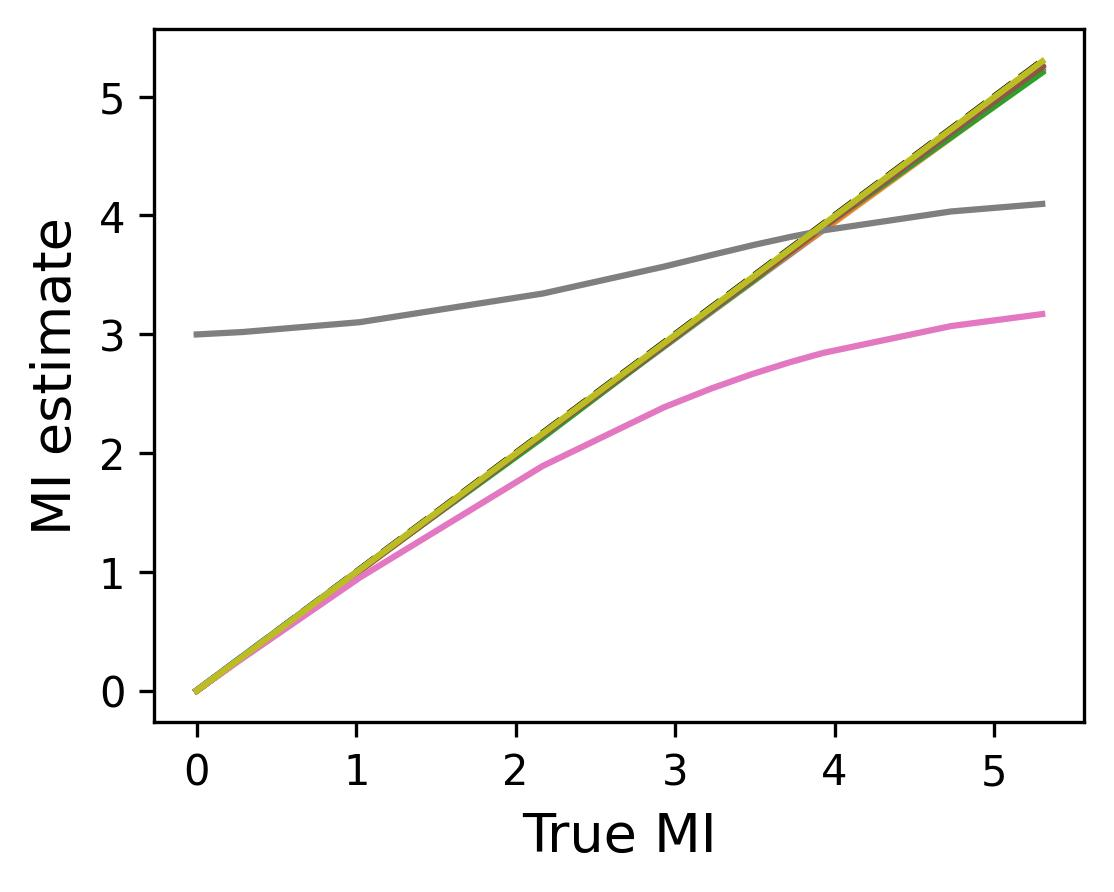
\includegraphics[page=1,width=\linewidth]{figures/high_mi_multinormal.jpg}
        \caption{Sparse Normal}
    \end{subfigure}
    \begin{subfigure}{0.25\textwidth}
        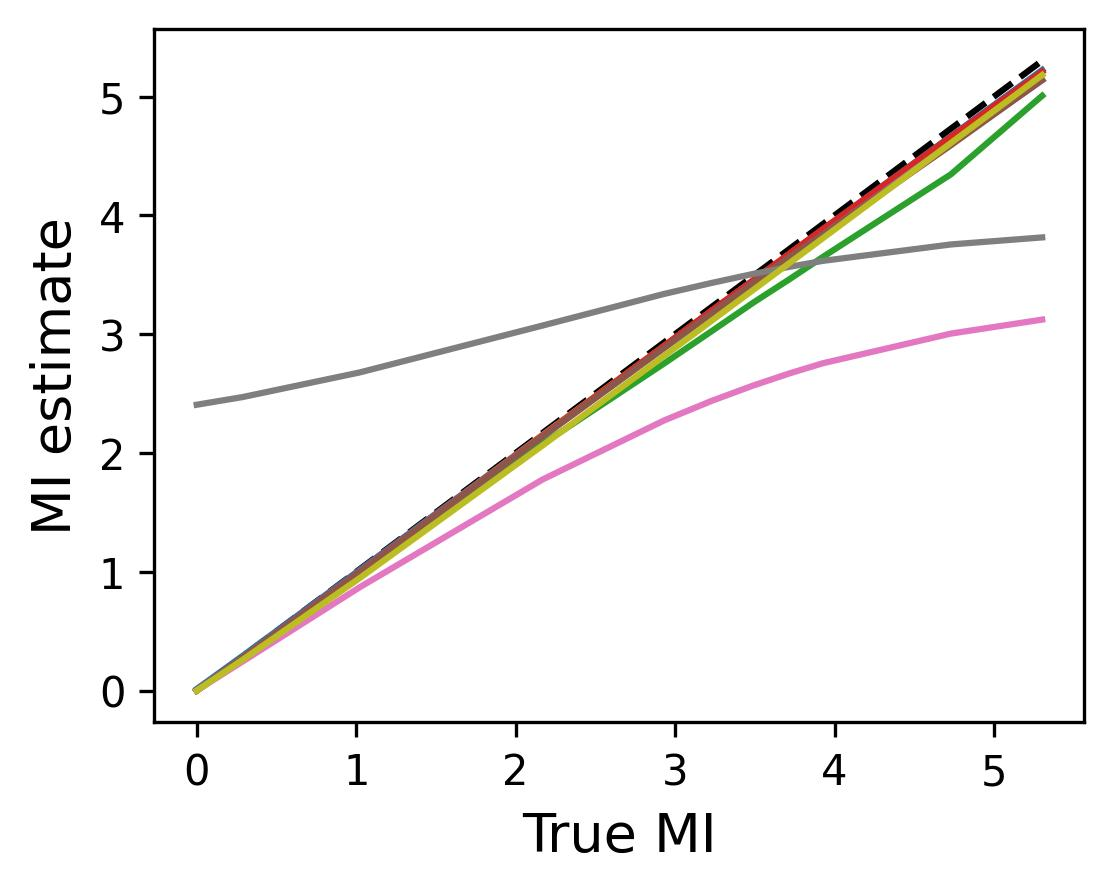
\includegraphics[page=1,width=\linewidth]{figures/Half-cube.jpg}
        \caption{Half-cube}
    \end{subfigure}
      \begin{subfigure}{0.25\textwidth}
        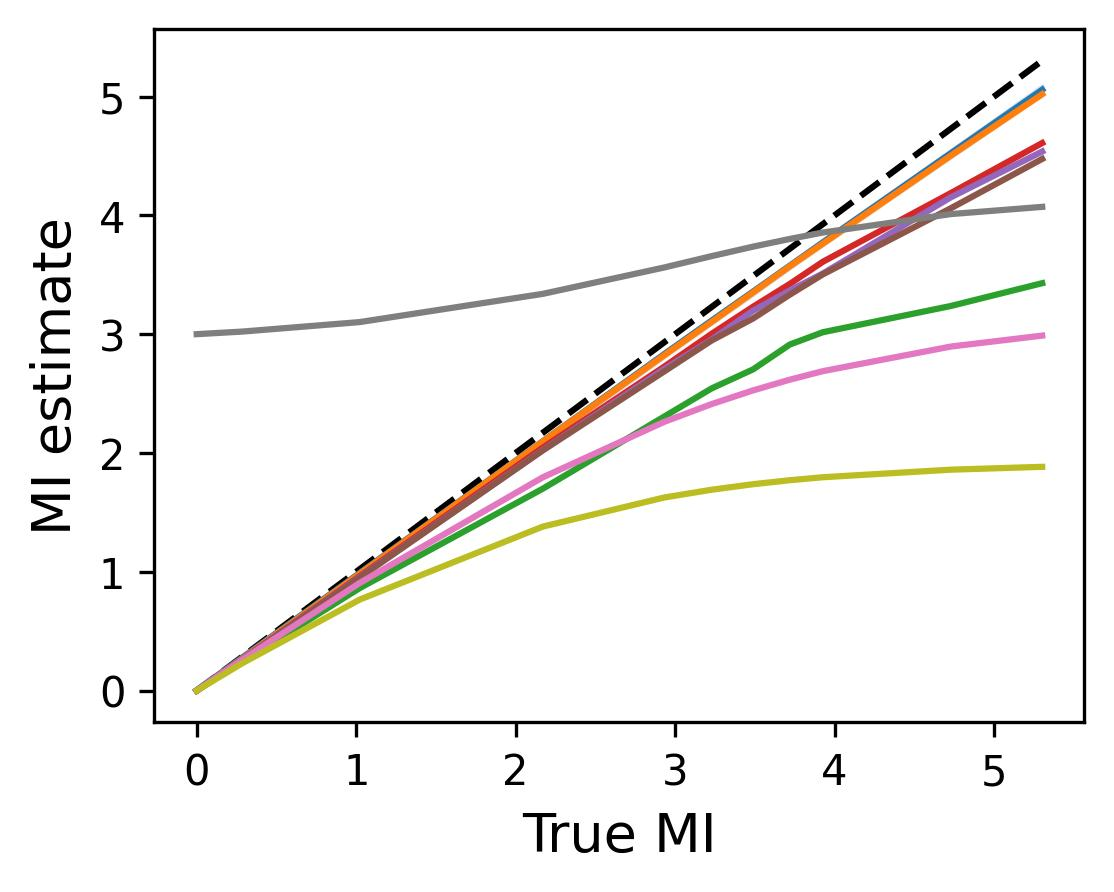
\includegraphics[page=1,width=\linewidth]{figures/spiral.jpg}
        \caption{Spiral  }
    
    \end{subfigure}
    \begin{subfigure}{0.1\textwidth}
        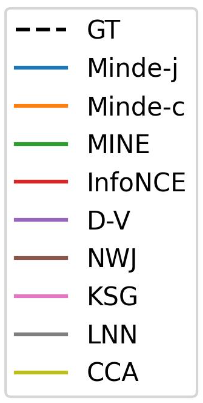
\includegraphics[page=1,width=\linewidth]{figures/legnd_final.png}
      
    \end{subfigure}
    \caption{original (a) and transformed variants ( (b) and (c)). 
     }
    \label{fig:high_mi}
\end{figure}

\framebreak
\item  Pass the self-consistency tests:
\begin{figure}[ht]
    \centering
        
    \begin{subfigure}{0.25\textwidth}
        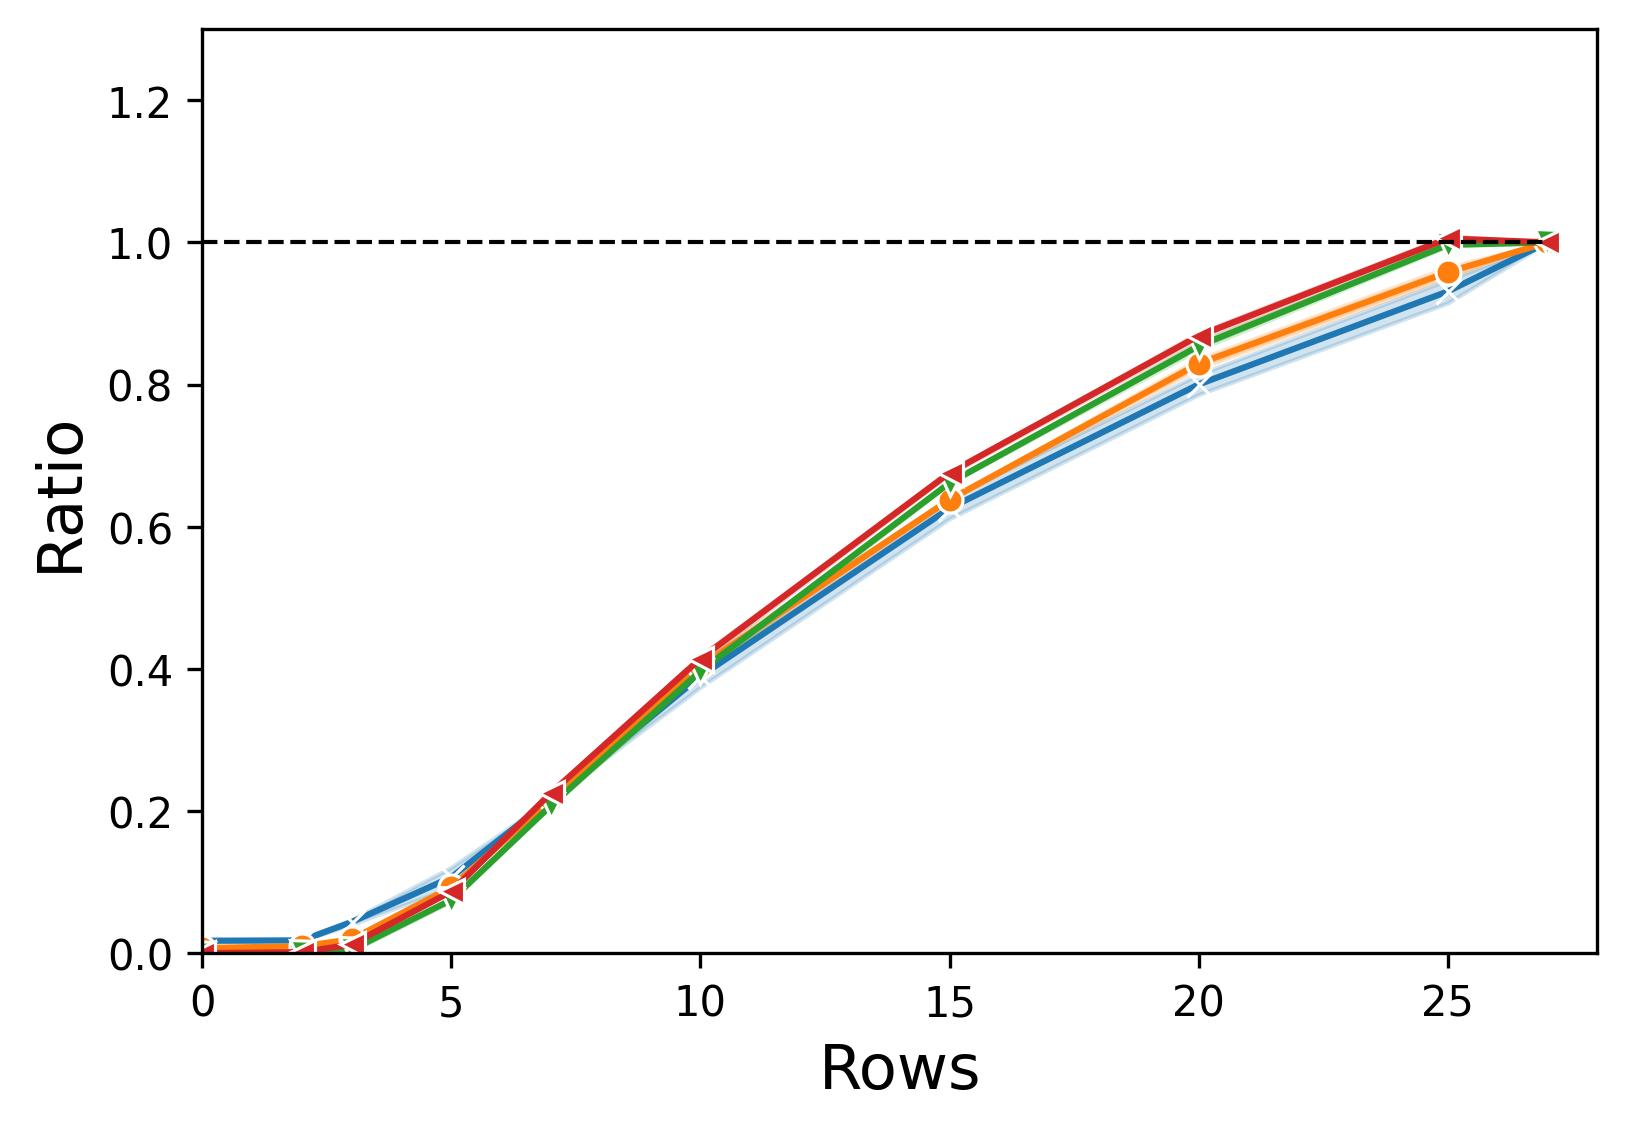
\includegraphics[page=1,width=\linewidth]{figures/consistency.jpg}
        \caption{ Baseline }
    \label{fig:set_1}\end{subfigure}
    \begin{subfigure}{0.25\textwidth}
        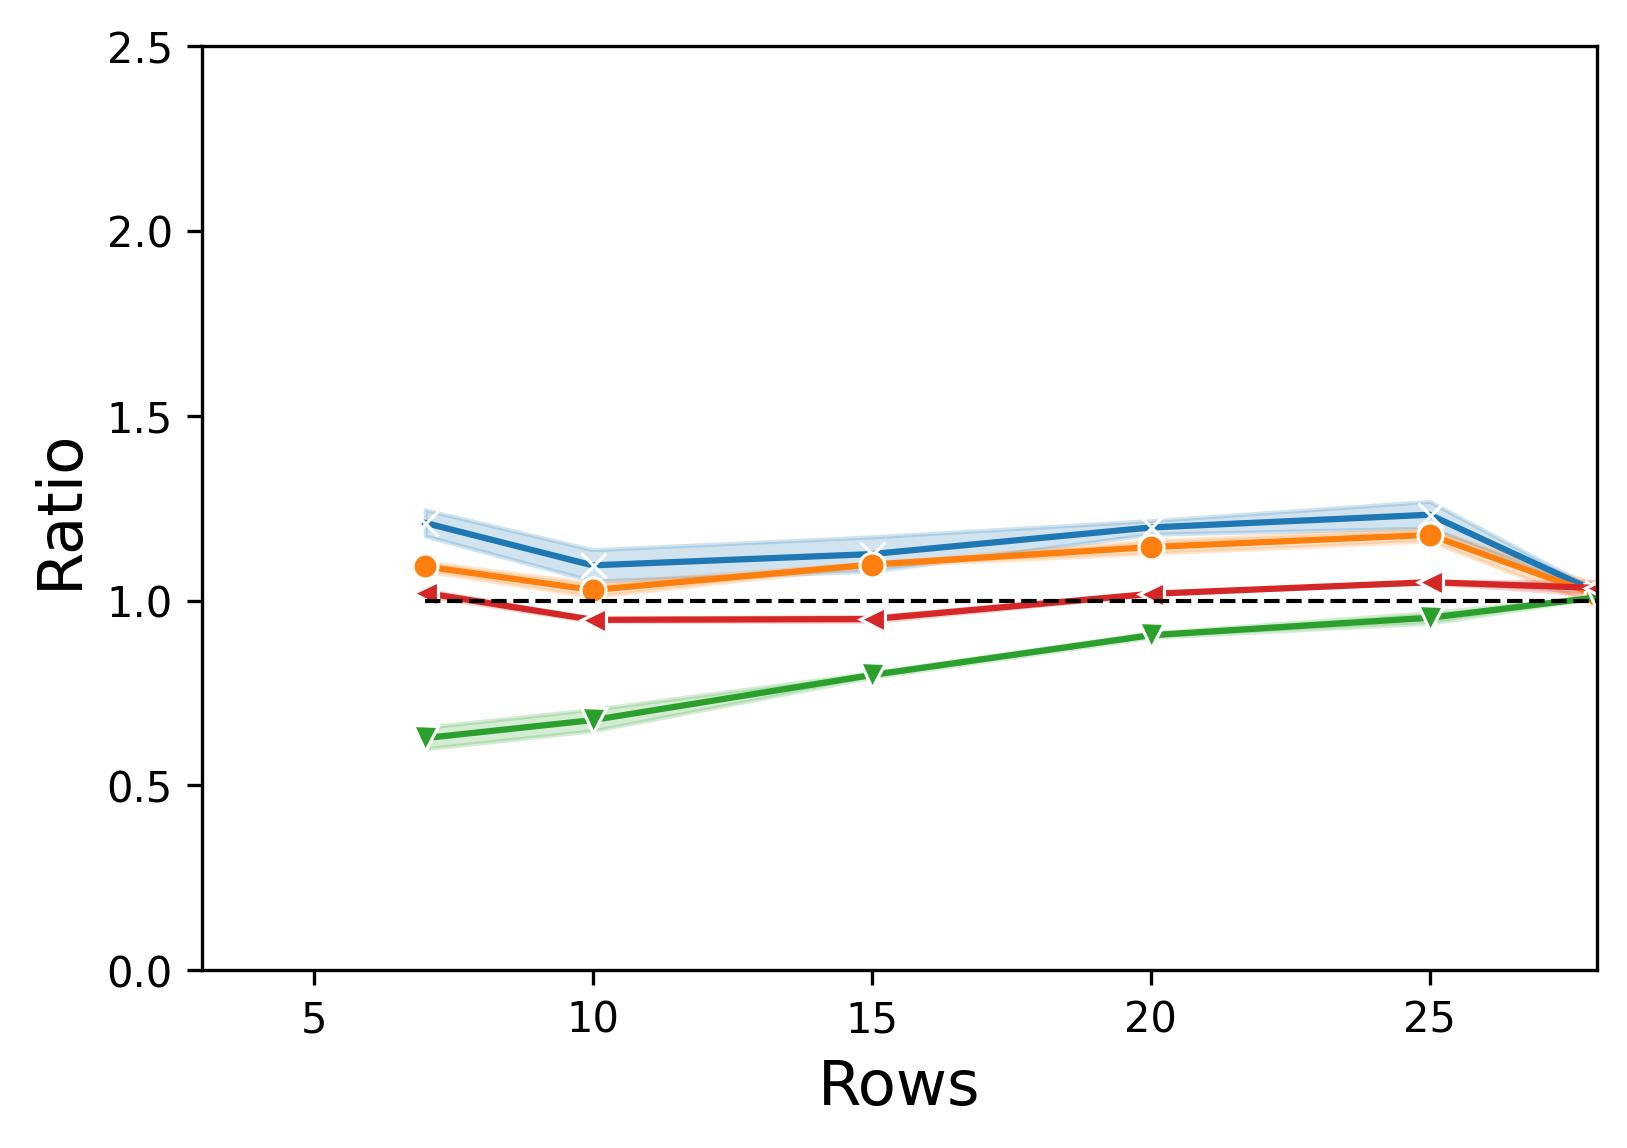
\includegraphics[page=1,width=\linewidth]{figures/dataprocessing.jpg}
        \caption{Data processing }
    \label{fig:set_2}
    \end{subfigure}
      \begin{subfigure}{0.25\textwidth}
        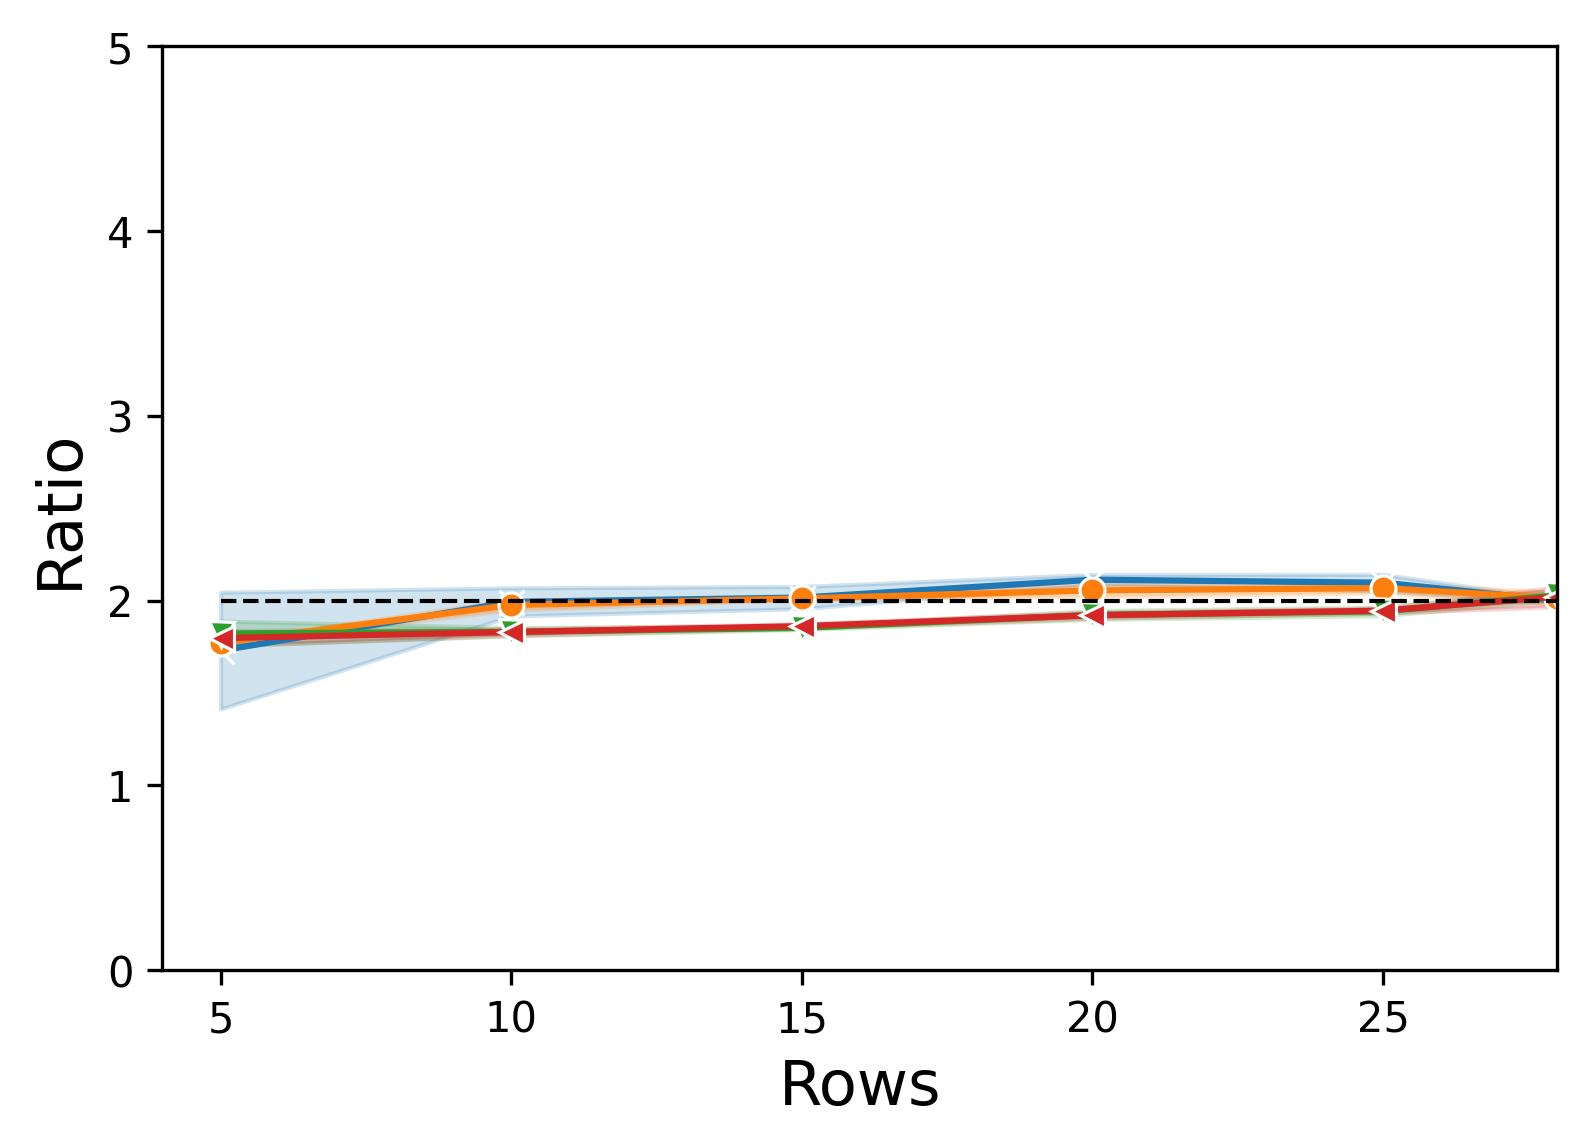
\includegraphics[page=1,width=\linewidth]{figures/additivity.jpg}
        \caption{Additivity  }
    \label{fig:set_3}
    \end{subfigure}
    \begin{subfigure}{0.15\textwidth}
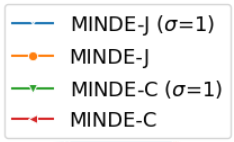
\includegraphics[page=1,width=\linewidth]{figures/legende.PNG}
          \caption*{  }
        \end{subfigure}
    \label{fig:consistency_rests}
\end{figure}
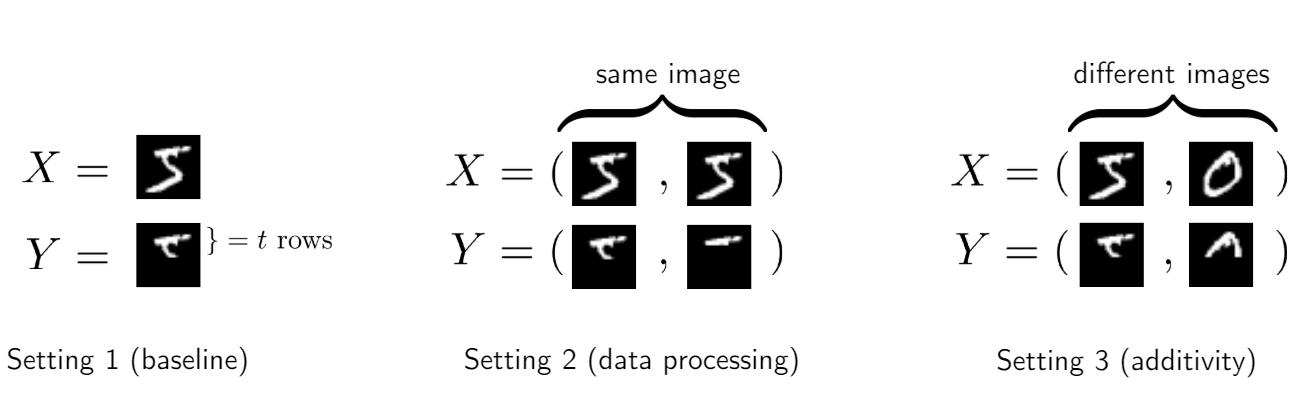
\includegraphics[width=\linewidth]{figures/consistency_tests.PNG}
\end{itemize}
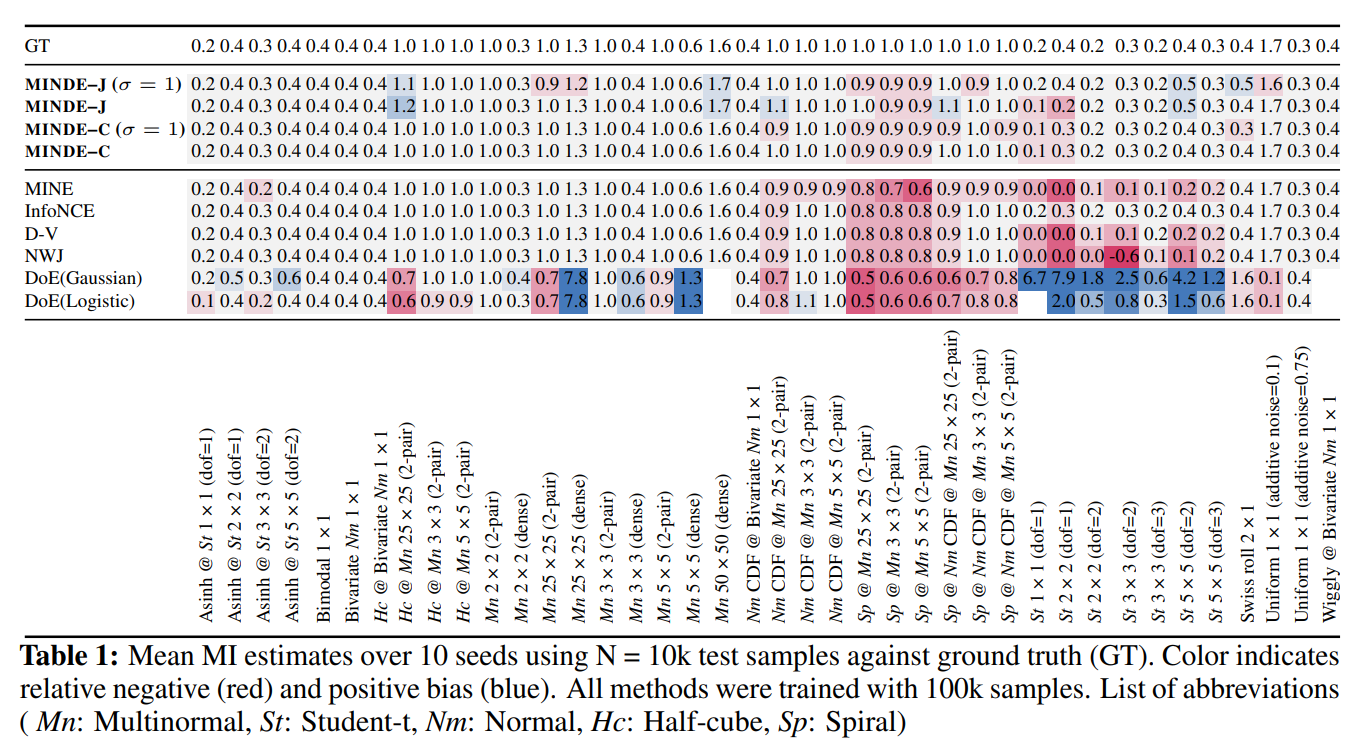
\includegraphics[scale=0.4]{figures/minde_res.PNG}

\end{frame}

\begin{comment}
\begin{frame}{Adaptation Filtration}
  
  \begin{itemize}
  \item   
  In this specific case, the process $Y_t$ is adapted to the filtration generated by $\sigma(Y_0, W_{0..t})$. In measurability terms, this means: "if I know $Y_0$ and $W_{0..t}$, I can numerically compute $Y_t$".
  \item In a constructive (but informal) way: 
  \begin{flalign*}
  &\sigma(Y_0,W_0)=\sigma(Y_0),\quad Y_0=\text{Id}(Y_0) \\ 
  &\sigma(Y_0,W_{0,...,\dd t})=\sigma(Y_0,\dd W_0 ),\quad Y_{\dd t}=Y_0+H_0(Y_0)\dd t+\dd W_0\\
  & \vdots
  \end{flalign*}
  
    \item Clearly, and almost tautologically, the process $Y_t$ is also adapted to its own filtration $\mathcal{F}^Y_t = \sigma(Y_s, s \leq t)$. If I know the full history of $Y_t$ up to time $t$, I can compute $Y_t$ itself.
    \item However, different filtrations correspond to different representations of the process.
  \end{itemize}
\end{frame}
\end{comment}

